\documentclass[letterpaper, oneside, 10pt]{report}
\usepackage[margin = 1.0in]{geometry}
\usepackage[nottoc,notlof,notlot]{tocbibind}
\usepackage[hidelinks]{hyperref}
\usepackage{graphicx}
\usepackage{amssymb}
\usepackage{epstopdf}
\usepackage{setspace}
\usepackage{wrapfig}
\usepackage{enumitem}
\usepackage{fancyhdr}
\usepackage{cite}
\usepackage{classicthesis}
\usepackage{caption}
\usepackage{subcaption}

\geometry{letterpaper}

\DeclareGraphicsRule{.tif}{png}{.png}{`convert #1 `dirname #1`/`basename #1 .tif`.png}

\setlength{\skip\footins}{0.8cm}
\setlength{\tabcolsep}{30pt}

% Title page parameters
\lhead{Andrew Lawson}
\title{\large COOPERATIVE 3-D MAP GENERATION USING MULTIPLE UAVS}
\author{
  \large
  Andrew Lawson \\
  University of Connecticut \\
  Computer Science and Engineering
}
\date{\large May 1, 2015}
\pagestyle{fancy}

\begin{document}

% Title page
\begin{titlepage}
  \maketitle
  \thispagestyle{empty}
\end{titlepage}
\clearpage

% Abstract
\begin{abstract}
  In the modern field of robotics, the ability for a robot to smoothly move about the environment, regardless of the medium, has proven to be fairly trivial. However, the ability for a mobile robot to track its own position and make deterministic decisions about it's own location in a foreign environment remains a fundamental, but critical problem. In most typical robotic experiments, the use of external measurement systems (such as GPS or motion capture cameras) allow researchers to capture the exact position of a robot in its environment and focus on other areas of interest. In the past couple decades, successful algorithms called SLAM\footnote{Simultaneous-Localization-And-Mapping: algorithm that uses sensor data to independently determine a position relational to an environment and simultaneously create a virtual map} have allowed singular mobile robots to determine their own position in a world space and construct a 3-D map from collected positional data. However, despite these advances, the ability for multiple UAV\footnote{UAV: unmanned aerial vehicle} robots to cooperatively determine their environmental boundaries is an area that remains relatively under-developed. Some studies have attempted this decentralized, cooperative approach, but fall short either by depending on external systems or lacking true 3-D capability. By taking this distributional approach with multiple robotic agents, the computational overhead of map generation is greatly reduced. Teams of coordinated robots could efficiently explore unaccessible areas, complete team-based tasks (like lifting large objects), conduct dangerous search and rescue missions, and ultimately increase the feasibility of robotics in numerous situations.
\end{abstract}
\clearpage

\renewcommand{\abstractname}{Acknowledgements}
\begin{abstract}
 I'd like to thank Prof. Shalabh Gupta, Prof. Ashwin Dani, and Prof. Robert McCartney for their advice and support. I'd also like to thank Kris Balisciano, Chung Yang, and everyone in L.I.N.K.S. Lab for all their work on the project.
\end{abstract}
\clearpage

% Table of Contents, Figures, and Tables
\tableofcontents
\listoffigures
\listoftables
\clearpage

\doublespacing

\chapter{Introduction}

\section{Overview}
\section{Literature Review}

In recent research projects with quadcopters, a wide variety of methods have been used to localize a robot in their environment, including (but not limited to) the use of high-resolution laser scanners \cite{bachrach2011range,shen2011autonomous}, monocular cameras \cite{soundararaj2009autonomous}, and ``RGB-D"\footnote{RGB-D: red-blue-green-depth} cameras as a combination of the two \cite{huang2011visual}. A laser has been used to generate a point cloud and pull out contours that trace the environment\cite{bachrach2011range}, a monocular camera to exploit texture gradients and continuations that can translated into depth estimates \cite{soundararaj2009autonomous}, and Microsoft Kinects (RGB-D cameras) to associate laser depth with image data \cite{huang2011visual}. Lasers capable of such precision and frequency are economically infeasible, and additionally, a pure visual approach is slow, can result in large margins of error, and lacks precision. Using a combination of the two, by means of an RGB-D camera, is responsive,  inexpensive, and produces results of reasonable reliability.


With previous RGB-D camera approaches, there have been five primary components: feature extraction, rotation estimation, feature matching, inlier detection, and motion estimation \cite{huang2011visual}. This involves taking certain features (like color, edges, corners, etc.) out of an image frame, estimating the rotation pose of the robot, matching new features to existing ones, filtering out bad data, and then estimating the motion of the robot. Using a data filter called an Extended-Kalman-Filter, the visual odometry data will be combined with velocity estimates to form a state estimation of the robot \cite{huang2011visual}. By implementing this filter, this will allow real-time positional estimates of the vehicle.


Researchers have also attempted de-centralized SLAM methods like I have proposed, but do not provide total three-dimensional capability. Some have used a VICON camera system \cite{leung2012decentralized} to provide true location data to robotic agents. Others have implemented truly autonomous, cooperative SLAM, but only focused on 2-D, planar data analysis \cite{cunningham2012large}. As I have mentioned previously, this does not fully address the ability to move and coordinate multiples robot entities independently in a realistic world setting. By examining this precedent work in the field, however, the ability to create cooperative 3-D SLAM can be fully visualized.

\chapter{Robot Design}

\section{Design Decisions}

Several key design decisions arose when choosing a direction for robot design and selection of components. The most signifcant choice for the robot was choosing an architecture for the onboard computational unit - specifically an ARM or x86 computer. The second key design dilemma involved the selection of a laser-scanning sensor or an RGB-D camera. As shown below, both these choices had great effect upon the path of experimentation and results obtained.

\subsection{ARM vs. x86}

The main advantage of choosing an x86 board (found in most desktop or laptop computers) is compatibility. Almost all software packages are available in prebuilt, binary form on package managers (such as Ubuntu's apt-get) and setting up the computing environment can be done with a few simple installation commands. This convenience, unfortunately, comes at a financial and dimensional price - most small form-factor x86 boards are extremely expensive and cheaper options are considerably larger in size. These tradeoffs make selection of such a board unfeasible for an aerial drone where space is extremely limited and minimization of cost is a primary concern. As a result, ARM boards (like those in smartphones) are much more attractive - they offer extremely small form-factors, yet remain very affordable. The issue that arises, of course, is that of compatibility - many programs or libraries are not (immediately) available on an ARM installation and require manual compilation of source code using an ARM-based compiler and possible changes to the source code itself first.

\subsection{Laser vs. RGB-D Camera}

\section{Hardware}

\subsection{Components}

The hardware design of the robot was focused on using low-cost, off-the-shelf components (see Table 1). The approximate cost of a built robot was \$894, significantly cheaper than pre-built alternatives such as the AscTec Pelican used at MIT \cite{bachrach2011range} and University of Washington \cite{bachrach2012estimation} with similar project requirements.

% Table of components used on robot
\begin{table}[h!]
  \centering
  \caption{Table of Components}
  \vspace{2mm}
  \begin{tabular}{l l l}
    \hline \hline
    \vspace{-2mm}
    Component & \multicolumn{1}{l}{Description} & \multicolumn{1}{l}{Cost} \\ [1ex]
    \hline
    & \\
    DJI F450 Frame & Chassis & \$200 \\
    DJI 1045 Propellers & Props & \$10 \\
    DJI 2212 Motors & Actuators & \$30 \\
    12V and 5V Regulators & Power Reg. & \$40 \\
    Zippy 2450 mAh LiPo & Battery & \$30 \\
    64GB ODROID XU3 & ARM SBU & \$240 \\
    Pixhawk PX4 & Controller & \$220 \\
    Microsoft Kinect & Visual Sensor & \$99 \\
    MaxSonar EZ0	& Sonar Sensor & \$25 \\
  \end{tabular}
\end{table}

\noindent The robot used a stock F450 frame from DJI, which was not modified in any way - all components were mounted on existing areas using screws or adhesive products.

\begin{figure}[h!]
 \caption{Photograph of finished quadcopter robot.}
 \centering
   \includegraphics[width=0.3\textwidth]{images/quadcopter}
\end{figure}

\noindent The onboard computational unit chosen was the ODROID XU3 by HardKernel, which has a 1.7Ghz quad-core Snapdragon CPU, 2GB DDR3 RAM, 64GB eMMC flash storage, USB 3.0, and draws 5A. Initially, the robot was equipped with a PandaBoard ES, possessing a 1.2Ghz dual core with 1GB DDR3 RAM, SD card storage, and drawing 3A. Due to low memory and high read/write latencies, the latter board struggled to bear the load of even a full Ubuntu installation and was replaced with the XU3. For the visual sensor, a stripped down Microsoft Kinect Model 1473 was mounted onto the quadcopter - removing the sensor housing reduced weight from a heavy 3 lb to a very nimble 100 g. A Pixhawk PX4 flight controller was also added to the system for actuation control - this allowed the focus of the project to remain on the mapping and flight components of the robot. To accomodate the 12V, 1A requirements of the Kinect and 5V, 5A of the ODROID, several power regulators were mounted and installed to the robot's power system. The entire system was powered by a single 2450 mAh LiPo battery.

\section{Software}

\subsection{ROS Hydro}

% ROS architecture
\begin{figure}[h!]
 \caption{Photograph of finished quadcopter robot.}
 \centering
   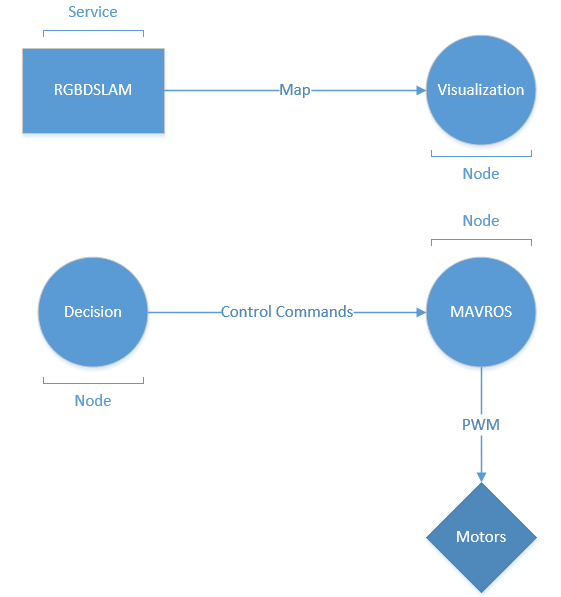
\includegraphics[width=0.4\textwidth]{images/ros_arch}
\end{figure}

\subsection{RGBDSLAM\_V2}
\noindent In order to compute a 3D map, the quadcopter's onboard computer uses an algorithm called SLAM (simultaneous localization and mapping) which computes a map and keeps track of the robotic agent's pose and translation relative to said map. Due to time constraints, it was decided that a proprietary SLAM algorithm was not an option and a previously developed software package was chosen instead. Due to it's compatibility with ROS and extensive accpetance throughout the robotics community, RGBDSLAM_V2 was the software used to produce the map and pose transformations of the robot during flight.

% RGBDSLAM data flow
\begin{figure}[h]
 \caption{Data flow of RGBDSLAM_V2}
 \centering
   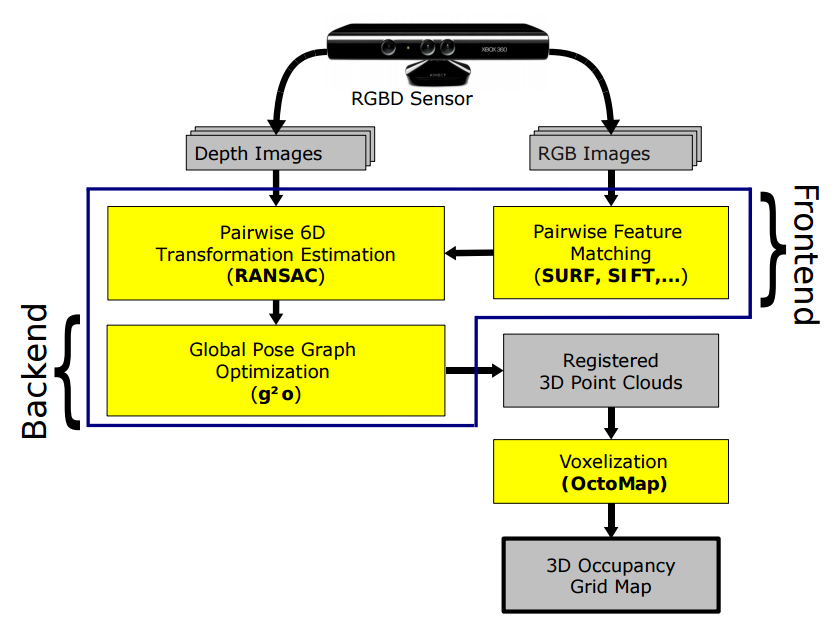
\includegraphics[width=0.6\textwidth]{images/rgbdslam}
\end{figure}

\subsection{MAVROS}

The direction of my project has two major stages to complete: Designing the robot and developing the navigation and map-building algorithms. \\

%\begin{figure}[h!]
 %\caption{Prototype quadcopter.}
 %\centering
   %\includegraphics[width=0.6\textwidth]{copter}
%\end{figure}

\chapter{Single Robot}

\section{Autonomy}
As the focus of this project is on the mapping component, fully-developed autonomous navigation is not present. However, some elements for inputless flight are implemented and provide a baseline for future work.

    \subsection{Pixhawk PID}
    The Pixhawk PX4 controller provides a built-in PID controller, which is used for drift stability and basic feedback control of the quadcopter. The proportional, integral, and derivative parameters were tuned through trial and error - adjusting each component until the quadcopter no longer oscillated and remained stable.

    \subsection{Altitude Control}

    The Pixhawk PX4 also provides an altitude holding system, given an input sensor.

\section{Mapping}

In a previous paper, Bachrach et al. implemented RGB-D mapping, and in a separate publication \cite{bachrach2011range}, laser mapping, by offloading realtime processing to a local server \cite{bachrach2012estimation}.  This robot design differs from its contemporaries by computing all steps of the mapping procedure onboard. As noted in Figure X, the quadcopter's onboard computer runs an RGBDSLAM ROS node in realtime during flight. This node generates the three-dimensional map, which can be be saved on disk as a file through a service call in ROS and retrieved after a test flight. The ROS node also allows requests for the current state of the map. As a result, a custom ROS node was written that allows for realtime visualization - this can be streamed to a nearby computer via Wi-Fi connection (see Figure X, Y). These two options allow for absolute flexibility in situations where remote access to the robot may or may not be possible.

\section{Results}
\noindent Testing of a single quadcopter robot was done in the concourse of the Information Technology Engineering building on the UConn Storrs campus. As seen in Figure 5, an image taken of the quadcopter in flight can be seen in the top left, the RGB stream from the Kinect sensor on the bottom left, and on the right-hand side, the 3-D map generated in realtime by the onboard computer.

% Map fusion algorithm flowchart
\begin{figure}[h]
 \caption{Live test of a single quadcopter.}
 \centering
   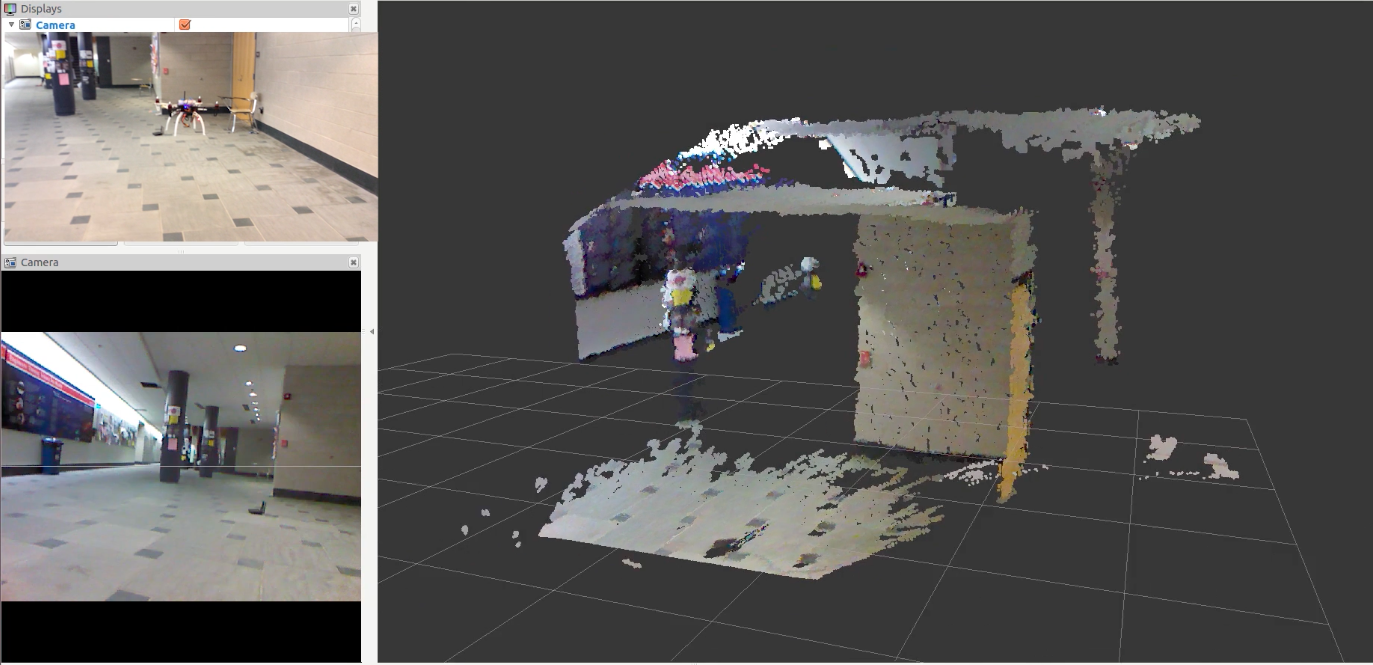
\includegraphics[width=0.8\textwidth]{images/single_test}
\end{figure}

\noindent Several repeated tests showed responsive mapping at about 7 frames per second. These maps were streamed in real time to a base station through a local wireless network.

\chapter{Multiple Robots}

\section{Overview}

\section{Online Mapping}
\noindent As discussed in the overview, each quadcopter needs to send its map over the network to be fused together. There are two primary methods to solve this, both with unique drawbacks. One such method is to deliver the entire aggregated point cloud map at given intervals to the server - this is immediately unfeasible because as time grows, the size of the map will grow to hundreds of megabytes and current network speeds are unable to process such a load in a reasonable time frame. The other solution is to send each individual point cloud corresponding to a timestep over the network, resulting in a reconstruction of the map on the server. This is inefficient, because the map has already been built onboard and it is redundant to perform the same operation remotely. The experiments in this report used the latter method despite its obvious weaknesses - it was the best choice given the constraints and time restrictions of the project.

Coupled with the mapping component of the RGBDSLAM_V2 package, a custom ROS node was written (integrated with RGBDSLAM_V2) that provided a stream of clouds added to the map, each corresponding to a new node added within the graph. As shown in figure X, these clouds are sent over the network and simultaneously received by a server or other external computer. For each cloud, the external computer also looks up the corresponding transformation between the fixed reference frame for the map and the current camera pose by listening to the transformation broadcaster within the RGBDSLAM_V2 algorithm. Once this transformation is received, it is applied to the new cloud, which is then concatentated to the current map.

% Networked map building algorithm flowchart
\begin{figure}[h]
 \caption{Live test of a single quadcopter.}
 \centering
   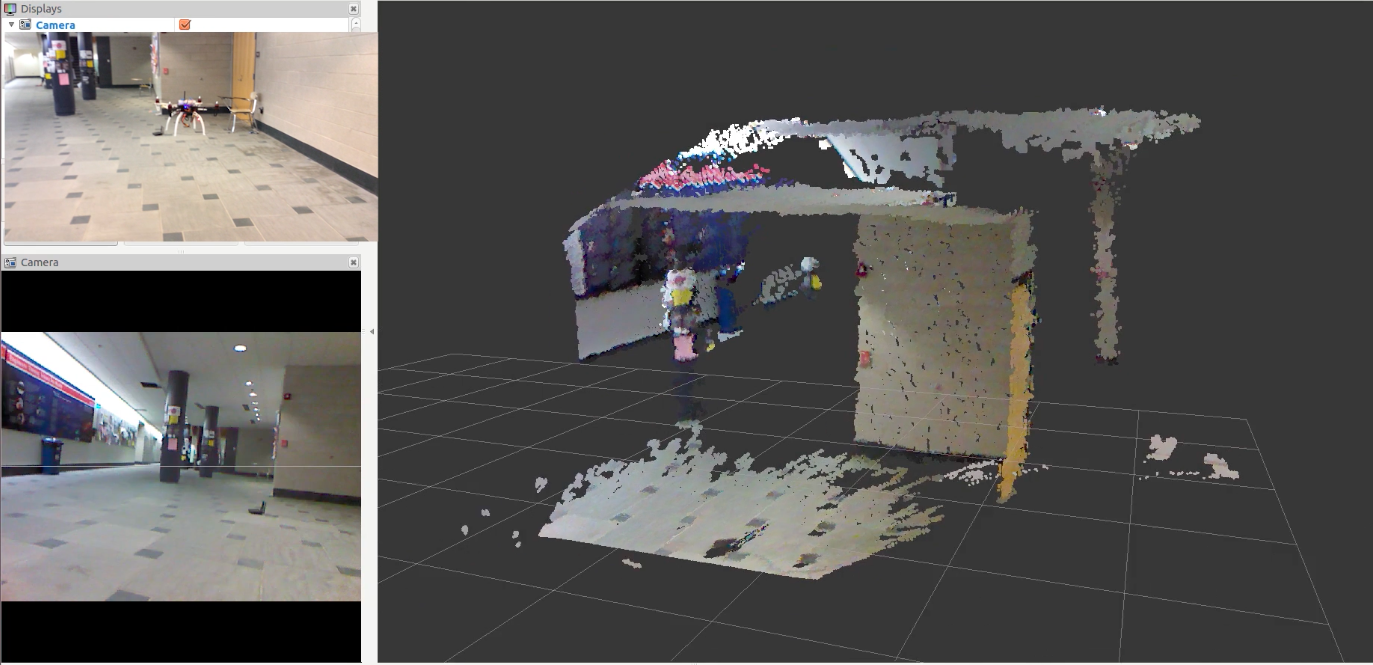
\includegraphics[width=0.8\textwidth]{images/single_test}
\end{figure}

\section{Map Fusion}
\noindent When transitioning from one robotic agent generating a global 3-D map to multiple robot agents, an algorithm capable of fusing each robot's local map together is essential. Each map generated by an individual robot has its own point cloud and pose (or transformation) in 3-D space. In order to make sense of these individual clouds, the algorithm accomplishes two goals: 1) it transforms two maps into the same global reference frame, 2) stitches the maps together and 3) eliminates redundant data points. By incrementally inputting maps into the algorithm, the server can output a final 3-D representative of all robotic agents' mapping efforts. As shown in Figure 2, this algorithm is divided into two key sections and follows a similar approach to Henry et. al.\cite{henry2012rgb}.

% Map fusion algorithm flowchart
\begin{figure}[h]
 \caption{Data flow of map fusion algorithm.}
 \centering
   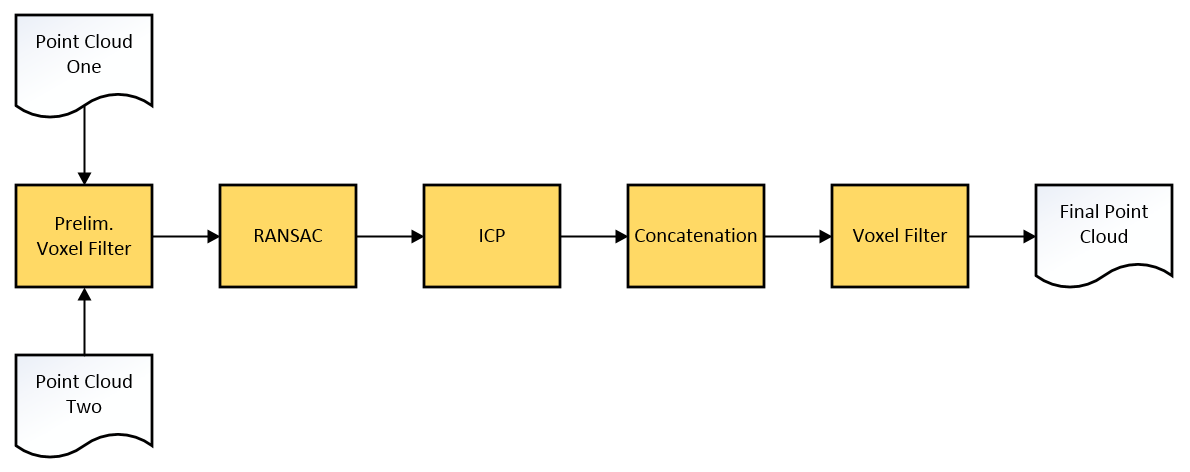
\includegraphics[width=0.9\textwidth]{images/mapfusion}
\end{figure}

    \subsection{Sample Consensus Initial Alignment}

    \noindent Given two maps within their own reference frame, it's necessary to transform the source map into the reference frame of the target map. The point clouds are first put through an initial alignment phase using the Sample Concensus Initial Alignment algorithm \cite{rusu2009fast}. This outputs a final transformation which is applied to the source cloud. In laymen's terms, this basically provides a large correction to the initial alignment of the two clouds, seen in Figure ~\ref{fig:Raw concatentation.}.

    \begin{figure}[h]
     \caption{Data flow of SCIA process.}
     \centering
       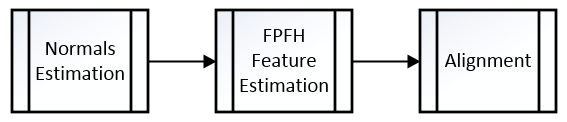
\includegraphics[width=0.45\textwidth]{images/initialalignment}
    \end{figure}

    \noindent Within the alignment process itself, there are several subprocesses. First, the normals $N_{source}$ and $N_{target}$ are found by PCL's normal estimator. These normal clouds are then used in PCL's Fast Point Feature Histogram (FPFH) \cite{rusu2009fast,rusu2009fastlabel} estimator, to generate approximate feature clouds $F_{source}$ and $F_{target}$. Lastly, these feature clouds from this process are used to estimate an initial transformation $T$, which is applied to the initial source cloud to obtain an initial alignment. This gives the clouds a reasonably close placement relative to each other, and allowing optimal usage of ICP in order to fine tune them.

    \subsection{Iterative Closest Point}

    \noindent After the clouds have passed through the initial alignment stage, they are locally optimized using the Iterative Closest Point algorithm. ICP takes a point cloud $P_{source}$ and finds the nearest neighbor points in $P_{target}$. By minimizing the sum of squares error, a rigid transformation $T$ between $P_{source}$ and $P_{target}$ is output. As shown in Figure ~\ref{fig:SCIA alignment.}, this transformation is applied to $P_{source}$ which eliminates narrower errors between the two clouds.

    \subsection{Filtering and Concatentation}

    Lastly, the target and transformed source cloud are concatenated using Point Cloud Library's concatentation features - programmatically, this is as simple as just adding the clouds together. Using another Voxel filter, the excess data points are trimmed away to generate the final stitched version of the map, as shown in Figure ~\ref{fig:ICP alignment.}. \\

% Map fusion visuals
\begin{figure}[h]
    \centering
    \begin{subfigure}[h]{0.31\textwidth}
        \centering
        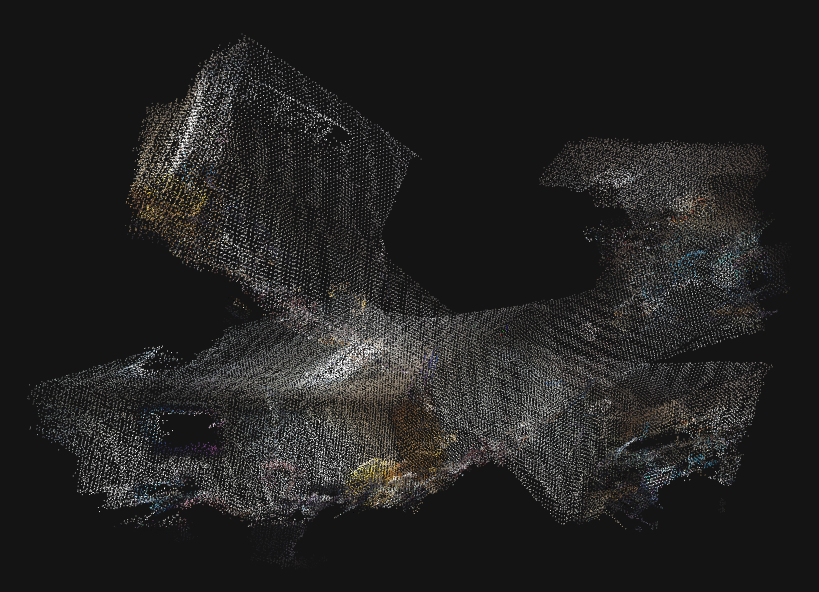
\includegraphics[width=\textwidth]{images/fusion_raw}
        \caption{Raw concatentation.}
        \label{fig:Raw concatentation.}
    \end{subfigure}
    \hfill
    \begin{subfigure}[h]{0.31\textwidth}
        \centering
        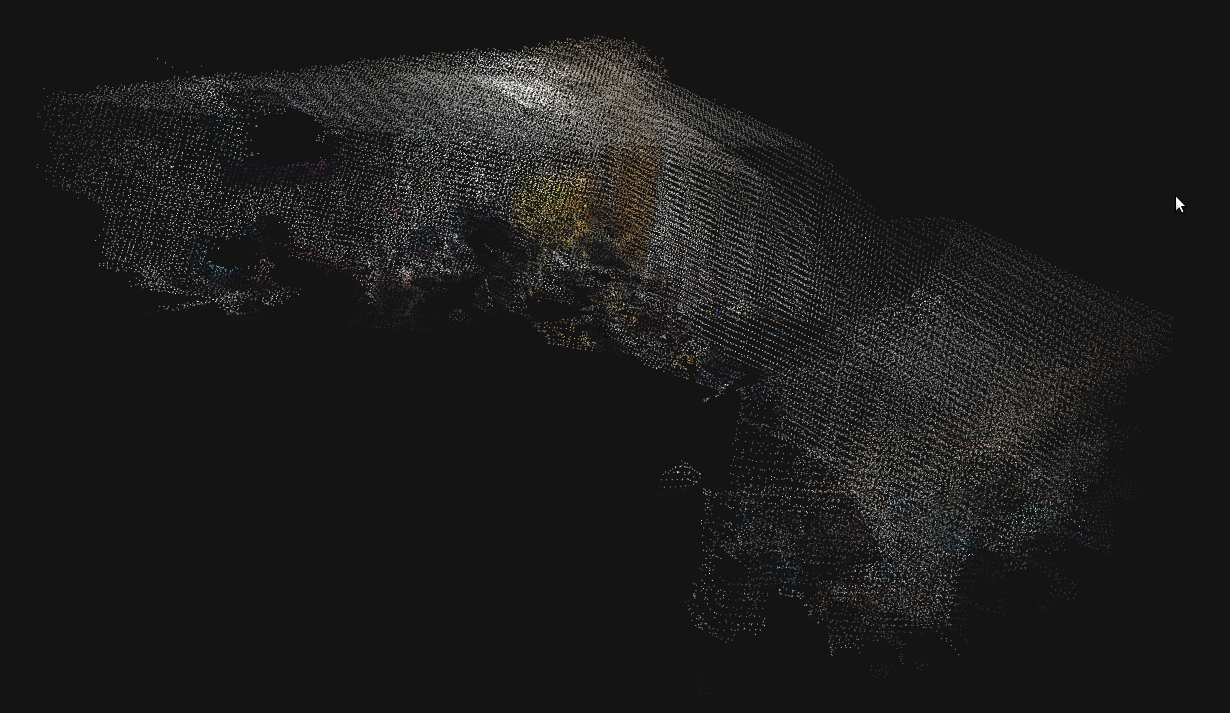
\includegraphics[width=\textwidth]{images/fusion_scia}
        \caption{SCIA alignment.}
        \label{fig:SCIA alignment.}
    \end{subfigure}
    \hfill
    \begin{subfigure}[h]{0.31\textwidth}
        \centering
        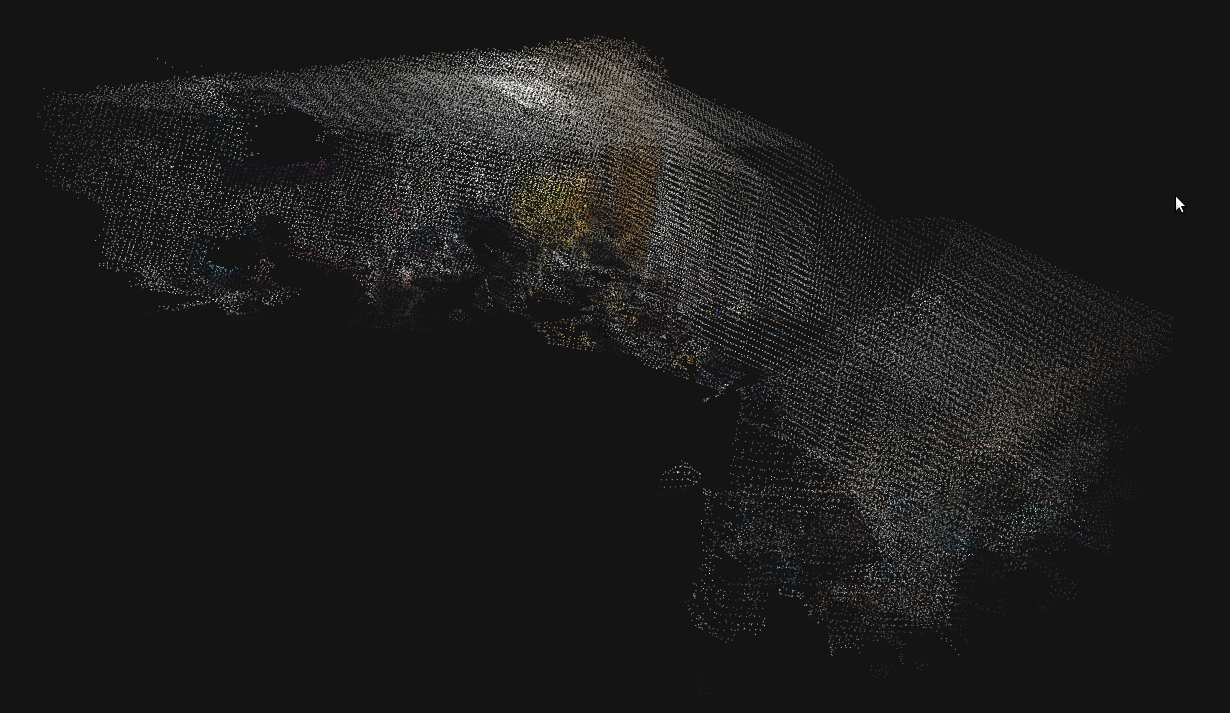
\includegraphics[width=\textwidth]{images/fusion_scia}
        \caption{ICP alignment.}
        \label{fig:ICP alignment.}
    \end{subfigure}
    \caption{Visual process of map fusion.}
    \label{fig:Visual process of map fusion.}
\end{figure}

\section{Results}

Due to financial and logistical difficulties, a test involving two quadcopters flying simultaneously in real time was unable to be conducted within the time frame for this project. As an alternative to demonstrate effectiveness of this approach, two separate flights using the same quadcopter were conducted in the same environment and saved into ROS bags. These ROS bags were then simulated as live nodes, with map data streaming at the same frequency and conditions as a real multi-robot flight test - this provided data to the map fusion server that exactly duplicates two quadcopters flying simultaneously and was an acceptable substitution for a real test.

\chapter{Conclusions}

\subsection{Future Work}

As stated earlier, this project did not focus on navigation or control of multiple quadcopters and took an interest purely within the feasibility of mapping using multiple quadcopters. A natural progression forward would be to implement localization and possible object avoidance. The RGBDSLAM algorithm was used exclusively for its mapping and pose graph features, but is also capable of estimating trajectory and facilitating autonomous navigation.

\chapter{Appendix}

% Table of PID parameters
\begin{table}[h!]
  \centering
  \caption{PID Parameters}
  \vspace{2mm}
  \begin{tabular}{l l}
    \hline \hline
    \vspace{-2mm}
    Parameter & \multicolumn{1}{l}{Value} \\ [1ex]
    \hline
    & \\
    Proportional & 0.05 \\
    Integral & 0.1 \\
    Derivative & 50 \\
  \end{tabular}
\end{table}

% Table of Map Fusion parameters
\begin{table}[h!]
  \centering
  \caption{Map Fusion Parameters}
  \vspace{2mm}
  \begin{tabular}{l l}
    \hline \hline
    \vspace{-2mm}
    Parameter & \multicolumn{1}{l}{Value} \\ [1ex]
    \hline
    & \\
    Voxel Leaf Size & 0.05 \\
    ICP Max. Corresp. Dist. & 0.1 \\
    ICP Max. Iter. & 50 \\
    ICP Trans. Epsilon & 1e-8 \\
    ICP Euclid. Epsilon & 1 \\
    SCIA Min. Sample. Dist & 1 \\
    SCIA Max. Corresp. Dist & 1 \\
    SCIA Max. Iter. & 50 \\
  \end{tabular}
\end{table}

\clearpage

\bibliography{uscholar}
\bibliographystyle{ieeetr}

\end{document}
